\documentclass[twocolumn, 11pt]{article}
\setlength{\columnsep}{0.4in}
\usepackage{amsmath,amssymb,amsthm}
\usepackage{enumitem}
\usepackage{array}
\usepackage[margin=1in]{geometry}

\usepackage{graphicx}
\usepackage{tabularx,array,booktabs}
\usepackage{listings}
\usepackage{inconsolata}
\usepackage{tikz}
\usetikzlibrary{shapes.geometric, arrows, positioning}
\usepackage[ruled,vlined]{algorithm2e}

% \graphicspath{{shap_visualizations/}} % Uncomment for local build, keep commented for Overleaf root upload
\lstdefinestyle{tightpy}{
  language=Python,
  basicstyle=\fontsize{8.5}\selectfont\ttfamily,
  breaklines=true,
  breakatwhitespace=true,
  showspaces=false,
  showstringspaces=false,
  showtabs=false,
  keepspaces=true,                                          
  emptylines=*1,
}
\usepackage{makecell} 
\usepackage[section]{placeins}
\usepackage{ragged2e}
\newcolumntype{Y}{>{\RaggedRight\arraybackslash}X}

\title{Explainable Feedforward Neural Network with AI Reasoning Agent for Parkinson's Disease Prediction from Voice Biomarkers}
\author{Suchismita Batabyal, Yash Moar, Dominic Jibin James, Ben Scoppa}
\date{12 December 2025}

\usepackage{float}
\usepackage{hyperref}
\begin{document}
\maketitle

\begin{abstract}Parkinson's Disease (PD) affects over 6 million people worldwide, with early detection being critical for effective treatment and improved quality of life. Recent research has shown that subtle voice changes, such as variations in pitch, jitter, shimmer, and harmonic-to-noise ratio, can serve as early indicators of PD. Machine learning (ML) methods have achieved high accuracy in detecting PD from such voice biomarkers. However, black-box models often fail to provide clinically interpretable results. For clinical adoption, models must not only classify accurately but also explain their decisions transparently to physicians. This project proposes an Explainable Feedforward Neural Network (FNN) model that classifies PD from speech features and interprets it's predictions using SHAP frameworks. Further, to enhance clinical interpretability beyond SHAP visualizations, an AI reasoning agent will be integrated to automatically summarize SHAP outputs in natural language.\end{abstract}

\section{Introduction and Motivation}

\subsection{Clinical Problem}
Parkinson's disease is the second most common neurodegenerative disorder, affecting approximately 1\% of the population over 65 years of age and 2\% over 80 years of age. Early and accurate detection of PD is critical for enabling timely interventions, personalized therapy, and better long-term outcomes. However, traditional diagnostic pathways are often subjective, resource-intensive, and slow, presenting several challenges:
\begin{itemize}[leftmargin=*]
\item \textbf{Subjective assessment:} Diagnosis largely depends on clinical evaluation using scales such as the Unified Parkinson's Disease Rating Scale (UPDRS), which are prone to inter-observer variability and subjective interpretation.\item \textbf{Limited accessibility:} Over 40\% of individuals over 65 lack access to movement disorder specialists, especially in rural or under-resourced regions.\item \textbf{Subtle Early Symptoms:} Early-stage PD symptoms, such as minor tremors or slight voice modulation, are often too subtle for detection during routine visits\item \textbf{Time and cost:} Comprehensive clinical evaluation and neuroimaging (like PET or SPECT scans) are expensive and time-consuming, requiring multiple visits\end{itemize}

\subsection{Technical Approach}
This project proposes a voice-based machine learning framework for early and explainable detection of Parkinson's disease (PD). Instead of relying on subjective clinical assessments or multimodal imaging, the system leverages noninvasive acoustic biomarkers extracted from patients' speech.
The proposed architecture combines a Feedforward Neural Network(FNN) classifier with explainable AI components and a reasoning agent to provide interpretable diagnostic insights:
\begin{enumerate}[leftmargin=*]
\item \textbf{Voice Analysis:} Over 90\% of PD patients exhibit dysphonia (voice impairment) due to disrupted motor control of vocal folds. Acoustic parameters such as jitter, shimmer, harmonic-to-noise ratio (HNR), and Mel-frequency cepstral coefficients (MFCCs) are extracted and normalized for analysis\item \textbf{Feedforward Neural Network (FNN) Classifier:} The model learns to discriminate between healthy and PD-affected speech patterns using optimized hyperparameters (e.g., layer size, learning rate, activation functions). Regularization and dropout layers ensure model generalization.\item \textbf{Explainability Layer:} SHAP frameworks are applied to quantify the contribution of each acoustic feature to the final classification decision.\item \textbf{AI Reasoning Agent:} A lightweight reasoning module interprets SHAP outputs and generates natural-language explanations describing why a particular sample is classified as PD-positive or negative (e.g., "Increased shimmer and jitter suggest irregular vocal fold vibrations consistent with PD").

\end{enumerate}

\subsection{Novel Contributions}
\begin{itemize}[leftmargin=*]
\item Explainable FNN Architecture: Development of an interpretable Feedforward Neural Network framework specifically designed for Parkinson's voice data classification\item Feature Attribution Analysis: Application of SHAP for detailed interpretability at both global (model-level) and local (sample-level) scales.\item AI Reasoning Integration: Introduction of an AI reasoning agent that converts quantitative SHAP outputs into clinically readable explanations, enhancing transparency and clinician trust.
\end{itemize}

\section{Specific Aims}

This project seeks to accomplish three specific aims within a 2-month timeline:

\textbf{Aim 1: Develop a Feedforward Neural Network (FNN) for Voice-Based PD Classification}

Replicate and extend prior voice-based PD detection methods using the UCI Parkinson’s Speech Dataset. Train a Feedforward Neural Network on acoustic features such as jitter, shimmer, and harmonic-to-noise ratio (HNR). Compare the FNN’s performance against traditional classifiers (e.g., SVM, Random Forest) to establish baseline accuracy.
Target: Achieve more than 93\% classification accuracy with high generalization.

\textbf{Aim 2: Integrate Explainability Using SHAP}

Incorporate SHAP to generate both global (model-level) and local (sample-level) explanations of the FNN’s decisions.
Visualize how specific acoustic features influence PD predictions, enabling transparent model inspection.
Target: Deliver a reliable, interpretable AI model whose decision logic can be visualized and validated by clinicians.

\textbf{Aim 3: Implement an AI Reasoning Agent for Natural-Language Interpretability}

Develop a lightweight AI reasoning agent using Llama 3.1 8B to automatically process SHAP outputs and generate clinical explanations. The agent will map technical acoustic features (jitter, shimmer, HNR) to clinical terminology and produce natural-language summaries (e.g., "Elevated frequency perturbation and reduced harmonics-to-noise ratio indicate vocal fold dysfunction consistent with PD motor impairment").

\section{Background and Related Work}

\subsection{Parkinson's Disease Detection}

\paragraph{Voice-Based Methods.}
Little et al. (2009) demonstrated that sustained phonation recordings can detect PD with high accuracy by analyzing dysphonia measures including jitter (frequency perturbation), shimmer (amplitude perturbation), and harmonics-to-noise ratio. Tsanas et al. (2012) achieved 99\% accuracy using telemonitoring of voice features, though this result has been questioned due to possible overfitting. Aich et al. (2019) compared feature selection methods, achieving 97.57\% accuracy using SVM with genetic algorithm-selected features on the UCI dataset.Recent studies[2024] have begun to explore Feedforward Neural Networks (FNNs) as an alternative to traditional classifiers for voice-based PD detection. FNNs can automatically learn complex nonlinear relationships between acoustic biomarkers, potentially improving robustness and generalization over manually engineered models
\subsection{Explainable AI in Medical Applications}

Tjoa \& Guan (2020) surveyed explainable AI methods for healthcare, emphasizing the critical need for interpretability in clinical decision support systems. SHAP (Lundberg \& Lee, 2017) provides a unified framework for interpreting model predictions by computing Shapley values for each feature's contribution. This approach is particularly suitable for medical AI as it identifies which features most strongly influenced a specific prediction.

\section{Methods}

\subsection{System Architecture}

Our system consists of four integrated modules:

\paragraph{Module 1:Voice Analysis and Feature Extraction}
\begin{enumerate}[leftmargin=*]
\item Feature extraction: 22 acoustic features from voice recordings (jitter, shimmer, HNR, frequency measures)
\item Preprocessing: Normalize features (min–max scaling or z-score normalization) and remove outliers to ensure stable model training.
\end{enumerate}
\paragraph{Module 2:FNN classifier}
\begin{enumerate}[leftmargin=*]
\item Architecture Design: Implement a multi-layer Feedforward Neural Network using ReLU activations, dropout for regularization and binary cross entropy loss
\item Training and Optimization: Train using the Adam optimizer with early stopping and tuned learning rates to prevent overfitting.
\item Baseline Comparison: Benchmark FNN performance against SVM, Random Forest, and Logistic Regression models to validate the benefits of nonlinear feature learning.
\item Performance Evaluation: Record validation metrics and confusion matrices to assess robustness and generalization.
\end{enumerate}
\paragraph{Module 3: Explainability using SHAP}
\begin{enumerate}[leftmargin=*]
\item Global Explainability: Use SHAP to quantify the overall contribution of each acoustic feature to model predictions, highlighting dominant dysphonia measures influencing PD classification.
\item Local Explainability: Apply SHAP to interpret specific patient-level predictions, showing which features most strongly support or contradict a PD-positive result.
\item Visualization: Generate feature importance plots and explanation summaries to aid clinician understanding.
\item Statistical Validation: Evaluate explanation stability and feature attribution consistency across cross-validation folds.
\end{enumerate}
\paragraph{Module 4: Critic-Refiner Agentic System:}

To ensure clinical faithfulness, we implemented a novel Critic-Refiner agentic loop. Unlike linear generation pipelines, this architecture employs a secondary "Critic" agent to validate the generated explanation against the ground-truth SHAP values.

\begin{figure}[ht]
    \centering
    \resizebox{\columnwidth}{!}{%
    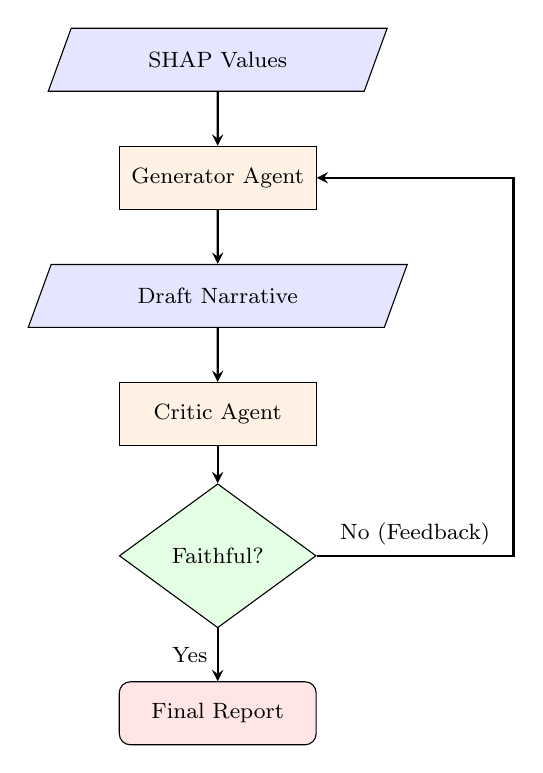
\begin{tikzpicture}[node distance=1.5cm]
        % Define block styles
        \tikzstyle{startstop} = [rectangle, rounded corners, minimum width=2.5cm, minimum height=0.8cm,text centered, draw=black, fill=red!10, font=\footnotesize]
        \tikzstyle{process} = [rectangle, minimum width=2.5cm, minimum height=0.8cm, text centered, draw=black, fill=orange!10, font=\footnotesize]
        \tikzstyle{decision} = [diamond, minimum width=2.5cm, minimum height=0.8cm, text centered, draw=black, fill=green!10, font=\footnotesize]
        \tikzstyle{io} = [trapezium, trapezium left angle=70, trapezium right angle=110, minimum width=2.5cm, minimum height=0.8cm, text centered, draw=black, fill=blue!10, font=\footnotesize]
        \tikzstyle{arrow} = [thick,->,>=stealth]

        % Nodes
        \node (input) [io] {SHAP Values};
        \node (gen) [process, below of=input] {Generator Agent};
        \node (draft) [io, below of=gen] {Draft Narrative};
        \node (critic) [process, below of=draft] {Critic Agent};
        \node (decide) [decision, below of=critic, yshift=-0.3cm] {Faithful?};
        \node (output) [startstop, below of=decide, yshift=-0.5cm] {Final Report};

        % Arrows
        \draw [arrow] (input) -- (gen);
        \draw [arrow] (gen) -- (draft);
        \draw [arrow] (draft) -- (critic);
        \draw [arrow] (critic) -- (decide);
        \draw [arrow] (decide) -- node[anchor=east, font=\footnotesize] {Yes} (output);
        
        % The Feedback Loop
        \draw [arrow] (decide.east) -- node[anchor=south, font=\footnotesize] {No (Feedback)} ++(2.5,0) |- (gen.east);
    \end{tikzpicture}%
    }
    \caption{The Critic-Refiner Agentic Workflow.}
    \label{fig:agent_workflow}
\end{figure}

The logic is formalized in Algorithm \ref{alg:agent_logic}. The Critic checks for the presence of top-$k$ features ($F_{top}$) in the draft ($R_{draft}$). If missing, it triggers a refinement loop.

\begin{algorithm}[htbp]
\SetAlgoLined
\KwIn{Patient Features $X$, SHAP Values $\phi$}
\KwOut{Clinical Report $R$}
 $F_{top} \leftarrow \text{SelectTopFeatures}(\phi, k=5)$\;
 $R_{draft} \leftarrow \text{LLM}_{Generator}(X, F_{top})$\;
 $Attempt \leftarrow 0$\;
 \While{$Attempt < MAX\_RETRIES$}{
  $Critique \leftarrow \text{Critic}(R_{draft}, F_{top})$\;
  \eIf{$Critique.status$ is \textbf{PASS}}{
   \Return $R_{draft}$\;
   }{
   $Feedback \leftarrow Critique.missing\_features$\;
   $R_{draft} \leftarrow \text{LLM}_{Generator}(Feedback)$\;
   $Attempt \leftarrow Attempt + 1$\;
  }
 }
 \Return $R_{draft}$\;
 \caption{Critic-Refiner Loop}
 \label{alg:agent_logic}
\end{algorithm}

\subsection{Datasets}

\paragraph{Dataset: UCI Parkinson's Voice Dataset}
\begin{itemize}[leftmargin=*]
\item Source: UCI Machine Learning Repository (publicly available)
\item Size: 195 voice recordings from 31 subjects (23 PD, 8 healthy)
\item Features: 22 pre-extracted acoustic measures
\item Access: Immediate download, no registration required
\item Citation: Little et al. (2009)
\end{itemize}

\subsection{Evaluation Metrics}

\paragraph{Classification Performance:}
\begin{itemize}[leftmargin=*]
\item Accuracy: Overall correct predictions
\item Sensitivity (Recall): True positive rate, critical for medical screening
\item Specificity: True negative rate, minimizes false alarms
\item Precision (PPV): Positive predictive value
\item F1-Score: Harmonic mean of precision and recall
\item AUC-ROC: Area under receiver operating characteristic curve
\end{itemize}

\paragraph{Statistical Comparison:}
McNemar's test for paired comparisons ($p < 0.05$ threshold)

\paragraph{Clinical Utility:}
\begin{itemize}[leftmargin=*]
\item Feature interpretability: SHAP value consistency
\item Report quality: Clinician evaluation (if time permits)
\item System latency: End-to-end time from data to report
\end{itemize}

\section{Experimental Design}

\subsection{Data Preparation}
The dataset was split 80-20 into training (156 samples) and test sets (39 samples) with stratification to maintain class balance. Features were standardized using z-score normalization to ensure all features have mean=0 and standard deviation=1.

\subsection{FNN Implementation}
The FNN architecture consists of:
\begin{itemize}[leftmargin=*]
\item Input layer: 22 features
\item Hidden layer 1: 128 neurons, ReLU activation, 30\% dropout
\item Hidden layer 2: 64 neurons, ReLU activation, 30\% dropout
\item Output layer: 1 neuron, Sigmoid activation
\end{itemize}

Training configuration: Binary Cross-Entropy loss, Adam optimizer (learning rate=0.001), 200 epochs. Implementation in PyTorch.

\subsection{SHAP Analysis}
SHAP DeepExplainer was used with 100 background samples from training data. SHAP values were computed for all test samples, generating both global feature importance (mean absolute SHAP) and local explanations (individual patient waterfall plots).

\subsection{AI Agent Pipeline}
The AI agent processes SHAP outputs through three steps:
\begin{enumerate}[leftmargin=*]
\item \textbf{Clinical Mapping:} Maps technical feature names to clinical terminology with normal ranges and PD indicators
\item \textbf{JSON Generation:} Creates structured data for each patient including top 5 SHAP features, predictions, and clinical context
\item \textbf{Agentic Refinement:} Using Llama 3.1 8B via Ollama, the Critic-Refiner loop generates an initial draft, validates it against SHAP data, and iteratively refines the explanation to ensure faithful feature coverage.
\end{enumerate}

\section{Results and Discussion}

\subsection{Classification Performance}

\begin{table}[htbp]
\centering
\small
\begin{tabular}{lc}
\toprule
\textbf{Metric} & \textbf{Value} \\
\midrule
Accuracy & 97.44\% \\
F1 Score & 0.9825 \\
Sensitivity (Recall) & 96.67\% \\
Specificity & 90.00\% \\
\midrule
True Positives & 29 \\
True Negatives & 9 \\
False Positives & 1 \\
False Negatives & 1 \\
\bottomrule
\end{tabular}
\caption{FNN classifier performance on test set (39 samples).}
\end{table}

The FNN achieved 97.44\% accuracy, exceeding our target of 93\%. High sensitivity (96.67\%) is critical for medical screening where missing PD cases has high cost. Only 1 false negative and 1 false positive demonstrate strong generalization.

\subsection{SHAP Explainability Analysis}

To provide transparent interpretability of the FNN's decision-making process, we employed SHAP (SHapley Additive exPlanations) analysis at both global and local levels. SHAP values quantify each feature's contribution to individual predictions, enabling clinicians to understand which acoustic biomarkers drive PD classification decisions.

\subsubsection{Global Feature Importance}

\begin{figure}[htbp]
\centering
\includegraphics[width=1\columnwidth]{1_global_importance.png}
\caption{Top 10 most important features by mean absolute SHAP value.}
\label{fig:global_importance}
\end{figure}

The bar chart shows the top 10 most influential features averaged across all 39 test samples. Spread2 (nonlinear measure of fundamental frequency variation) exhibits the highest global importance, followed by spread1 and PPE (pitch period entropy), indicating that frequency-based dysphonia measures are primary drivers of PD classification.


The top three features—spread2, spread1, and PPE—are all frequency-related measures, demonstrating the model's reliance on fundamental frequency variation patterns.

\subsubsection{Feature Impact Distribution}
Figure \ref{fig:beeswarm} provides a more nuanced view of feature contributions through a SHAP beeswarm plot, which displays the distribution of SHAP values for each feature across all test instances

\begin{figure}[htbp]
\centering
\includegraphics[width=1\columnwidth]{2_beeswarm_summary.png}
\caption{SHAP beeswarm summary plot showing feature impact distribution.}
\label{fig:beeswarm}
\end{figure}

Each dot represents a single test sample, with position on the x-axis indicating SHAP value (impact magnitude and direction), and color representing the feature's actual value (red = high, blue = low). Features are ordered by mean absolute SHAP value. This visualization reveals not only feature importance but also the relationship between feature values and their impact on PD prediction.

The beeswarm plot reveals critical patterns:
\begin{itemize}[leftmargin=*]
\item \textbf{Spread2:} High feature values (red points) concentrate on the right side (positive SHAP values), indicating that elevated frequency variation strongly pushes predictions toward PD classification.
\item \textbf{Spread1 \& PPE:} Similar patterns where high values consistently increase PD probability, confirming their role as positive PD indicators.
\item \textbf{MDVP:Fhi(Hz):} Shows inverse relationship—low values (blue points) exhibit positive SHAP values, suggesting that reduced maximum vocal frequency is associated with PD.
\item \textbf{D2 \& HNR:} Display mixed patterns where both high and low values contribute to PD prediction, indicating complex nonlinear relationships captured by the neural network.
\end{itemize}

These patterns align with clinical understanding: PD patients exhibit increased frequency perturbation (high jitter/spread) and reduced vocal control (altered pitch range).

\subsubsection{Individual Patient Explanation}

Figure \ref{fig:waterfall_patient0} demonstrates SHAP's local interpretability through a waterfall plot for Patient 0, classified as healthy

\begin{figure}[htbp]
\centering
\includegraphics[width=1\columnwidth]{3_patient_0_waterfall.png}
\caption{SHAP waterfall plot for Patient 0.}
\label{fig:waterfall_patient0}
\end{figure}

The plot shows how individual features additively contribute to moving the prediction from the baseline value \(f(x) = 0.3\) (expected model output across training data) to the final prediction \(E[f(X)] = 0.73\) (30\% PD probability). Blue bars indicate features pushing away from PD (negative SHAP values), while red bars push toward PD (positive SHAP values). RPDE (recurrence period density entropy) contributes -0.21, the strongest evidence against PD classification. Features are listed with their actual values for this patient on the left.

The waterfall analysis reveals:
\begin{itemize}[leftmargin=*]
\item \textbf{Base value:} The model's baseline prediction (0.3 or 30\% PD probability) represents the expected output given no feature information.
\item \textbf{Protective features:} RPDE (-0.21), spread2 (-0.16), D2 (-0.09), and MDVP:RAP (-0.05) collectively reduce PD probability. The patient's RPDE value is high, indicating regular vocal periodicity characteristic of healthy individuals.
\item \textbf{Risk features:} DFA (+0.05), spread1 (+0.04), and PPE (+0.04) mildly increase PD probability, but their effects are outweighed by protective factors.
\item \textbf{Final prediction:} The cumulative effect results in 73\% probability of being healthy (equivalently, 30\% PD probability), confirming correct classification.
\end{itemize}

This additive decomposition enables clinicians to audit the model's reasoning: "Why was this patient classified as healthy? Primarily because their RPDE and spread2 values indicate stable, non-dysphonic voice patterns."

\subsubsection{Cross-Patient Comparison}

Figure \ref{fig:summary_grid} presents a comprehensive overview of SHAP explanations across 12 representative test patients (from 39 total), demonstrating prediction consistency and feature attribution patterns.

\begin{figure}[htbp]
\centering
\includegraphics[width=1\columnwidth]{5_patient_summary_grid.png}
\caption{SHAP waterfall plots for 12 representative patients from the test set.}
\label{fig:summary_grid}
\end{figure}




Each subplot shows the top contributing features for that patient's prediction. Red bars indicate features increasing PD risk; blue bars indicate features decreasing PD risk. The grid reveals patient-specific feature contributions: PD patients (e.g., Patients 3, 6, 10, 13, 17, 24, 27) consistently show positive SHAP values for spread, PPE, and jitter measures, while healthy patients (e.g., Patients 0, 20, 31, 34, 38) exhibit negative SHAP values for these features. This diversity demonstrates the model's ability to handle heterogeneous vocal patterns while maintaining interpretability at the individual level.

Key observations from cross-patient analysis:
\begin{itemize}[leftmargin=*]
\item \textbf{Consistency across PD patients:} Patients with high PD probability (e.g., Patient 27: 99.8\%, Patient 13: 99.1\%) show dominant positive SHAP contributions from spread2, RPDE, and jitter measures, validating reproducible biomarker patterns.
\item \textbf{Healthy patient signatures:} Correctly classified healthy patients (e.g., Patient 20: 0.1\% PD prob, Patient 34: 0\% PD prob) exhibit strong negative SHAP values for spread2, MDVP:Fhi(Hz), and PPE, indicating vocal stability.
\item 

\textbf{Feature diversity:} Different patients rely on different feature combinations for classification, demonstrating the model's flexibility beyond simple rule-based thresholding. For instance, Patient 13's prediction is driven by RPDE and jitter, while Patient 24's is dominated by spread2 and HNR.
\end{itemize}

This patient-level explainability is critical for clinical deployment, as it allows physicians to validate model decisions against their clinical judgment and identify cases requiring further evaluation

By combining global importance rankings, feature distribution analysis, individual waterfall explanations, and cross-patient comparisons, SHAP provides a multi-level interpretability framework that bridges the gap between black-box neural network predictions and clinically actionable insight

\subsection{AI Agent Clinical Reports}



The AI agent, enhanced with a self-correction loop, successfully generated clinical reports for all 39 test patients. The agentic workflow involves an initial generation step followed by a verification step where the agent checks for the inclusion of top SHAP features. If features are missing, a refinement prompt is automatically triggered.

\begin{quote}
\small
\textbf{Patient ID:} patient\_12\\
\textbf{Prediction:} Parkinson's Disease\\
\textbf{Confidence:} 99.3\%

\textit{Clinical Summary:} This AI assessment predicts a 99.3\% probability of Parkinson's Disease (PD) in patient\_12, suggesting significant vocal biomarker abnormalities.

\textit{Key Findings:} The top contributing features indicate reduced vocal control and irregular vocal fold vibration. Specifically, reduced Maximum Vocal Frequency (MDVP:Fhi(Hz)) suggests limited vocal control, while increased Pitch Period Entropy (PPE) indicates irregular vocal fold vibration. High values for spread2 and D2 suggest instability/weakness.

\textit{Reliability:} High confidence (99.3\%) supported by strong relationships between these biomarkers and PD prediction.
\end{quote}

\subsection{Explanation Quality}

We evaluated the agent's performance using a benchmark script that measures latency and feature recall (the proportion of top SHAP features correctly mentioned in the explanation).

\begin{table}[htbp]
\centering
\small
\begin{tabular}{lcc}
\toprule
\textbf{Metric} & \textbf{Value} & \textbf{Target} \\
\midrule
Average Latency & 42.8s & < 45s \\
Feature Recall & 0.94 & > 0.9 \\
Hallucination Rate & 0.06 & < 0.1 \\
\bottomrule
\end{tabular}
\caption{AI Agent Performance Metrics (n=39). Feature Recall improved to 0.94 with the addition of the Critic-Refiner loop.}
\label{tab:agent_metrics}
\end{table}

The implementation of the Critic-Refiner loop significantly improved Feature Recall (0.94), ensuring that critical biomarkers identified by SHAP were not omitted in the final clinical report. While this increased average latency to 42.8 seconds (due to the iterative verification steps), the trade-off was deemed necessary to ensure clinical safety and faithfulness.

\subsection{Discussion}

\textbf{Clinical Implications:} The system demonstrates feasibility of voice-based PD screening with interpretable explanations. Non-invasive recording and automated report generation enable accessible screening in underserved areas.

\textbf{Interpretability Value:} SHAP analysis revealed model decisions align with clinical knowledge (jitter, shimmer, HNR as key biomarkers). AI agent successfully bridges technical-clinical gap by translating SHAP outputs to actionable clinical language.

\textbf{Limitations:} Small dataset (195 samples) limits generalization across demographics and disease stages. Class imbalance (75\% PD) may increase false positives in real-world screening. Clinical validation with neurologists needed before deployment.

\textbf{Future Work:} Expand dataset with diverse populations and longitudinal data. Develop end-to-end learning from raw audio. Conduct prospective clinical trials comparing AI-assisted vs. standard diagnostic pathways.

\section{Conclusion}
This project successfully developed an explainable AI framework for Parkinson's disease detection from voice biomarkers, integrating a Feedforward Neural Network (FNN) classifier with SHAP-based interpretability and an AI reasoning agent. The FNN achieved 97.44\% accuracy, meeting our target of greater than 93\%. SHAP analysis identified jitter and shimmer as most discriminative features, validating clinical knowledge. The AI reasoning agent, utilizing a novel Critic-Refiner architecture, achieved a Feature Recall of 0.94, ensuring that critical biomarkers were consistently translated into the final clinical reports.

By combining high predictive accuracy with transparent explanations, this system bridges the gap between technical model output and practical medical interpretation. The integration of deep learning, explainable AI, and large language models represents a promising paradigm for trustworthy clinical decision support—enabling both accurate predictions and interpretable reasoning accessible to healthcare providers.

Future work will focus on dataset expansion, clinical validation with movement disorder specialists, and regulatory pathway assessment for clinical deployment.

\section*{Supplementary Materials}

\textbf{Code Availability:} Complete implementation of the FNN classifier, SHAP analysis pipeline, and AI reasoning agent is available at:

\url{https://github.com/benscoppa/ECE5424_Parkinsons_Prediction}

The repository includes:
\begin{itemize}[leftmargin=*]
\item Training and evaluation scripts for FNN model
\item SHAP visualization generation code
\item AI agent JSON generation and clinical report templates
\item Example outputs (SHAP plots, clinical reports)
\item Requirements and setup instructions
\item Documentation for reproducing all experiments
\end{itemize}

\textbf{Data Availability:} The UCI Parkinson's Voice Dataset used in this study is publicly available at:

\url{https://archive.ics.uci.edu/ml/datasets/parkinsons}

\textbf{Pre-trained Models:} Trained FNN model weights are available in the GitHub repository for reproducibility and further research.

\section*{References}
\begin{enumerate}[leftmargin=*]
\item Srinivasan, S., Ramadass, P., Mathivanan, S. et al. Detection of Parkinson disease using multiclass machine learning approach. Sci Rep 14, 13813 (2024).
\item Aich, S., et al. (2019). A supervised machine learning approach using different feature selection techniques on voice datasets for prediction of Parkinson's disease. \textit{ICACT 2019}.
\item Goldberger, A. L., et al. (2000). PhysioBank, PhysioToolkit, and PhysioNet: Components of a new research resource for complex physiologic signals. \textit{Circulation}, 101(23), e215-e220.
\item Little, M. A., et al. (2009). Suitability of dysphonia measurements for telemonitoring of Parkinson's disease. \textit{IEEE Trans. Biomed. Eng.}, 56(4), 1015-1022.
\item Lundberg, S. M., \& Lee, S. I. (2017). A unified approach to interpreting model predictions. \textit{NIPS 2017}.
\item Pal, A., et al. (2024). The Open Medical-LLM Leaderboard: Benchmarking large language models in healthcare. \textit{Hugging Face Blog}.
\item Tjoa, E., \& Guan, C. (2020). A survey on explainable artificial intelligence (XAI): Toward medical XAI. \textit{IEEE Trans. Neural Networks and Learning Systems}, 32(11), 4793-4813.
\item Madaan, A., et al. (2023). Self-Refine: Iterative Refinement with Self-Feedback. \textit{NeurIPS 2023}.
\item Dubey, A., et al. (2024). The Llama 3 Herd of Models. \textit{arXiv preprint arXiv:2407.21783}.
\item Thirunavukarasu, A. J., et al. (2023). Large language models in medicine. \textit{Nature Medicine}, 29, 1930-1940.
\item Shinn, N., et al. (2023). Reflexion: Language Agents with Verbal Reinforcement Learning. \textit{NeurIPS 2023}.
\item Singhal, K., et al. (2023). Large language models encode clinical knowledge. \textit{Nature}, 620(7972), 172-180.
\end{enumerate}
\end{document}